\chapter{Marco teórico} % Main chapter title

\label{ch:MarcoTeorico} % For referencing the chapter elsewhere, use \ref{Chapter1} 

%----------------------------------------------------------------------------------------


La Web contiene una gran cantidad de opiniones respecto a productos, políticos, y mucho mas, expresado en forma de noticias, sitios de opinión, reseñas en tiendas online, redes sociales. Como resultado, el problema de ``Minería de opinión'' ha obtenido una atención creciente en las ultimas dos décadas y es un factor decisivo para las nuevas organizaciones (como es mencionado en \cite{Popescu2007}). De esto mismo partimos que el análisis de textos para extraer el significado y demás componentes extraíbles del texto componen un factor que debe considerarse al momento de realizar decisiones, de manera que los avances hechos hasta ahora tienen como meta una aplicación practica de lo que se conoce como \glsentrylong{nlp}.

Luego de los ataques terroristas del 11 de Septiembre de 2001 en Estados Unidos, se realizaron fuertes criticas respecto a la inteligencia, donde el director del FBI~\emph{Robert~S.~Mueller} indico que el principal problema que la agencia tuvo fue que se enfocaba demasiado en lidiar con el crimen luego de que fue cometido y ponía muy poco énfasis en prevenirlo (adaptado de \cite{mena2003investigative}). Es por esto que el uso de \gls{nlp} para temas de seguridad como también de metodologías de \glsentrylong{machinel} y \glsentrylong{deepl} han sido ampliamente utilizadas en ámbito de seguridad luego de estos eventos.

Para obtener una mejor inteligencia se necesito de mejores tecnologías a las que se tenían entonces (véase \cite[p\'ag 2]{mena2003investigative}):
\begin{itemize}
\item Integración de datos (\'o \gls{dataintegration} en ingl\'es)
\item Análisis de vínculos (\'o \gls{linkanalisys} en ingl\'es)
\item Agentes de software (\'o \gls{softwareagents} en ingl\'es)
\item Minería de texto (\'o \gls{textmining} en ingl\'es)
\item Redes neuronales (\'o \gls{neuralnetworks} en ingl\'es)
\item Algoritmos de \glsentrylong{machinel} (\'o \gls{mlalgorithms} en ingl\'es)
\end{itemize}

% ================================================================

\section{Análisis de vínculos (\glsentrylong{linkanalisys})}
Es la visualización de asociaciones entre entidades y eventos, por lo general involucran una visualización por medio de una gráfica o un mapa que muestre las relaciones entre sospechosos y ubicaciones, sea por medio físico o por comunicaciones en la red.

% ================================================================

\section{Agentes de software (\glsentrylong{softwareagents})}
Es el software que realiza tareas asignadas por el usuario de manera autónoma, donde sus habilidades básicas son:
\begin{itemize}
\item \textbf{Realización de tareas:} Hacen obtención de información, filtrado, monitoreo y reporte.
\item \textbf{Conocimiento:} Pueden usar reglas programadas, o pueden aprender reglas nuevas (véase \ref{sec:KBS}).
\item \textbf{Habilidades de comunicación:} Reportar a humanos e interactuar con otros agentes.
\end{itemize}

% ================================================================

\section{Sistemas Basados en Conocimiento (\glsentrylong{kbs})} \label{sec:KBS}
Según \cite{sajja2010knowledge}, los \gls{kbs} son uno de los mayores miembros de la familia de \gls{ai}. El \gls{kbs} consiste de una \gls{knowledgebase} y un programa de búsqueda llamado \gls{inferenceengine} representado en la figura \ref{fig:kbs-arch}. La \gls{knowledgebase} puede ser usado como un repositorio de conocimiento de varias formas.

Existen 5 tipos de \gls{kbs}, donde uno de ellos es conocido como \gls{expertsystems}, donde su uso se da como \gls{rulebasedsys}, donde su \gls{knowledgebase} esta dado como reglas y su \gls{inferenceengine} esta dado por algo llamado \gls{workingmemory}, que representa los hechos que se conocen inicialmente del sistema junto con los hechos que se van dando como inferencia de las reglas.

\begin{figure}[th]
\centering
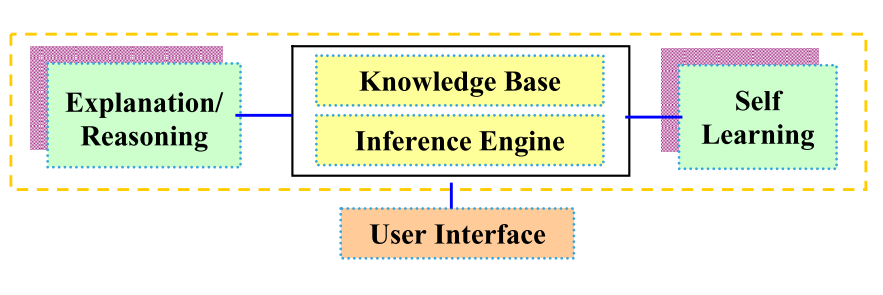
\includegraphics[scale=0.4]{Figures/kbs-architecture.png}
\decoRule
\caption[Arquitectura \glsentrytext{kbs}]{Arquitectura \glsentrytext{kbs}. Tomado de \cite{sajja2010knowledge}}
\label{fig:kbs-arch}
\end{figure}

Estas reglas pueden resumirse como una colección de condicionales de la forma \textbf{IF/ELSE} que se componen de un \emph{antecedente} y un \emph{consecuente}.

Existen dos tipos de \gls{rulebasedsys}, definidos como \gls{deductivesys} y \gls{reactivesys}, donde el \gls{deductivesys} tiene como objetivo realizar una conclusión en base a los hechos iniciales en la \gls{workingmemory}, por el otro lado se tienen los \gls{reactivesys}, los cuales de igual manera a los \gls{deductivesys}, toman los hechos de la \gls{workingmemory} y realizan sea una acción interactiva con su entorno o bien una modificación de los hechos que se encuentran en la \gls{workingmemory} tal como la adición o eliminación de hechos. Tómese el ejemplo de la ecuación \ref{eq:rbs-example} tomada de \cite{Mendel}, donde \emph{x} es la temperatura y \emph{AC} es aire acondicionado.

\begin{equation} \label{eq:rbs-example}
  \left\{ \begin{array}{ll}
            \text{IF x es moderado,} & \text{THEN y = ajustar AC a bajo} \\
            \text{IF x es alto,}     & \text{THEN y = ajustar AC a moderado a alto} \\
            \text{IF x es muy alto,} & \text{THEN y = ajustar AC a alto} 
          \end{array} \right.
\end{equation}

\subsection{Fuzzy Knowledge Based Systems}
Pendiente

% ================================================================

\section{Mineria de texto (\glsentrylong{textmining})} \label{sec:NLP}
Es un subcampo de Inteligencia Artificial conocida como \glsentrylong{nlp}, en donde las herramientas de minería de datos pueden capturar rasgos críticos del contenido de un documento basado en el análisis de sus características lingüísticas.

La mayoría de los crímenes son electrónicos por naturaleza, por lo que se dejan rastros textuales que investigadores pueden seguir y analizar. Estas se enfocan en el descubrimiento de relaciones en texto no--estructurado y pueden ser aplicados al problema de \emph{búsqueda} y \emph{localización de palabras clave}.

% ================================================================

\section{Redes Neuronales (\glsentrylong{neuralnetworks})} \label{sec:NN}
Pendiente

\subsection{Sistemas de Detección de Anomalías (\glsentrylong{anomalydetectionsys})}
Pendiente

\subsection{Mapa autoorganizado (\glsentrylong{som})}
El objetivo principal de los \gls{som} es de transformar una patrón de entrada $m$--dimensional en un mapa discreto uni-- o bi--dimensional, donde sus principales características es que es un algoritmo que se basa en \gls{unsupervisedl}, es \gls{feedforward}, es de una sola capa de neuronas donde su propósito es de realizar \gls{clustering} y realizar una reducción de dimensionalidad sobre los datos de una forma topologicamente ordenada.

Los \gls{som} tienen tres características distintivas:
\begin{itemize}
\item {\bf Competencia:} por cada patrón de entrada, las neuronas en la red competirán entre ellas para determinar un ganador.
\item {\bf Cooperación:} la neurona ganadora determina la ubicación espacial (vecinos) alrededor de donde otras vecinas también se verán estimuladas.
\item {\bf Adaptación:} la neurona ganadora como también sus vecinas tendrán sus pesos asociados actualizados, y se tiene que los vecinos entre mas cerca estén del ganador, mayor es el grado de adaptación.
\end{itemize}

El algoritmo de aprendizaje de \gls{som} parte de primero inicializar los pesos de las $o$ neuronas con pesos aleatorios pequeños de una distribución de probabilidad aleatoria o uniforme, donde cada vector de entrada se define como $x = [x_1, \ldots, x_m]^{T} \in \mathbb{R}^{m}$ y la entrada general de $N$ patrones como $\mathbf{X}^{m \times N}$, el vector de pesos de la neurona $i$ es $\mathbf{w}_i = [w_{i1}, \ldots, w_{im}] \in \mathbb{R}^{l \times m}$, con la matriz de pesos $\mathbf{W}^{o \times m}$.

Para alcanzar el objetivo de \emph{competencia}, se realiza por cada patrón de entrada $x_i$ una comparación con cada uno de los pesos de las $o$ neuronas y se establece la de menor distancia respecto $x_i$ (típicamente la distancia Euclidiana), dejando un ganador $winner$, tal como en la ecuación \ref{eq:som-competition}.
\begin{equation} \label{eq:som-competition}
  winner = \text{argmin}_j \norm{x_i - w_j} ; j = 1, \ldots,o
\end{equation}

Luego de establecer la neurona ganadora, se realiza el paso para alcanzar la \emph{cooperación}, que consiste en que por medio de una función kernel $h$ (típicamente una una distribución gaussiana), que permite establecer un área de afectación de las otras neuronas según su ubicación física en el mapa, definidos como $r_{winner}$ y $r_j$ que son la ubicación de la neurona ganadora y la neurona vecina $j$, en el cual el grado de afectación de la neurona vecina depende de la distancia de la que esta de la neurona ganadora, definido en la ecuación \ref{eq:som-cooperation}.
\begin{equation} \label{eq:som-cooperation}
  h_{j, winner}(t) = \text{exp}\Bigg(\frac{- \norm{r_j - r_{winner}}^2}{ 2 \sigma(t)^2}\Bigg)
\end{equation}

Parte importante del proceso de convergencia del \gls{som} es que a medida que avanzan las iteraciones $t$ del algoritmo el área de afectación se va reduciendo como parte del proceso de adaptación, por lo que definimos $\sigma(t) = \sigma_0 \text{exp}(-t / \tau_1)$, donde $\tau_1$ es una constante heurística y $\sigma_0$ la dimensión del mapa \gls{som}.

Finalmente para alcanzar la \emph{adaptación} se realiza una actualización de los pesos de la matriz $\mathbf{W}$ en base a la influencia de área $\sigma(t)$ y de una tasa de aprendizaje $\alpha(t) = \alpha_0 \text{exp}(-t/ \tau_2)$, donde $\tau_2$ es otra constante heurística y $\alpha_0$ es una constante de aprendizaje inicial, que debe ser $0 \le \alpha_0 \le 1$, la actualización se describe por la ecuación \ref{eq:som-adaptation} y el proceso puede ser visto gráficamente en la figura \ref{fig:som-adap-proc}, tanto de forma uni-- como bi--dimensional.
\begin{equation} \label{eq:som-adaptation}
  w_j(t+1) = w_j(t) + \alpha(t) h_{j, winner}(t)\Big[x_i-w_j(t)\Big]
\end{equation}

\begin{figure}[th]
\centering
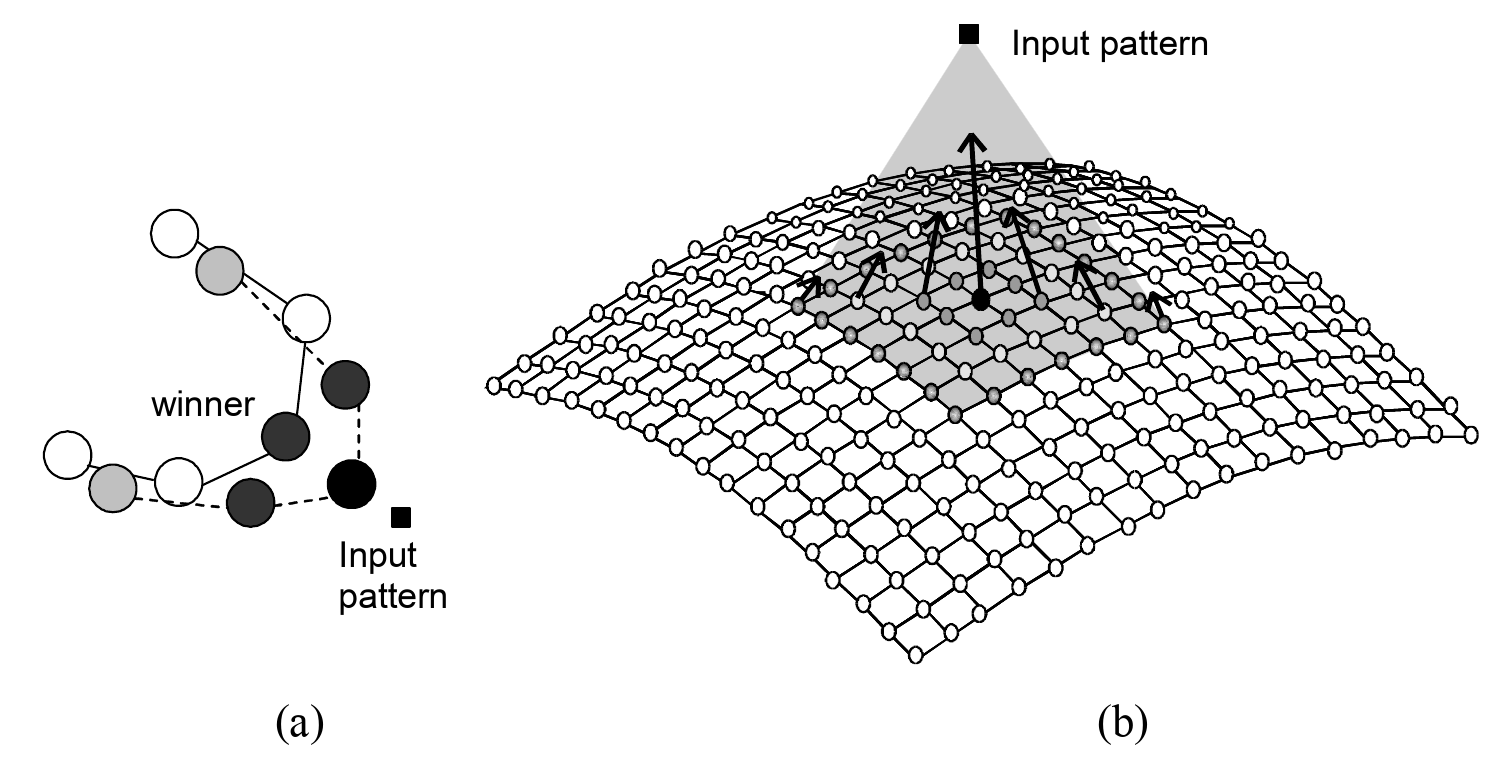
\includegraphics[scale=0.2]{Figures/som-adaptive-proc.png}
\decoRule
\caption[Proceso de adaptación de \glsentrytext{som}]{Proceso de adaptación de \glsentrytext{som}, (a) uni--dimensional, (b) bi--dimensional. Tomado de \cite{de2006fundamentals}}
\label{fig:som-adap-proc}
\end{figure}

Luego de que el algoritmo de aprendizaje termina de realizar las iteraciones, la salida de este es la matriz de pesos $\mathbf{W}$, en la figura \ref{fig:som-impl-example} se puede apreciar una aproximación del algoritmo con un mapa uni--dimensional tratando de aproximar una función sinusoidal con ruido adicionado en un gráfico 2D.

\begin{figure}[th]
\centering
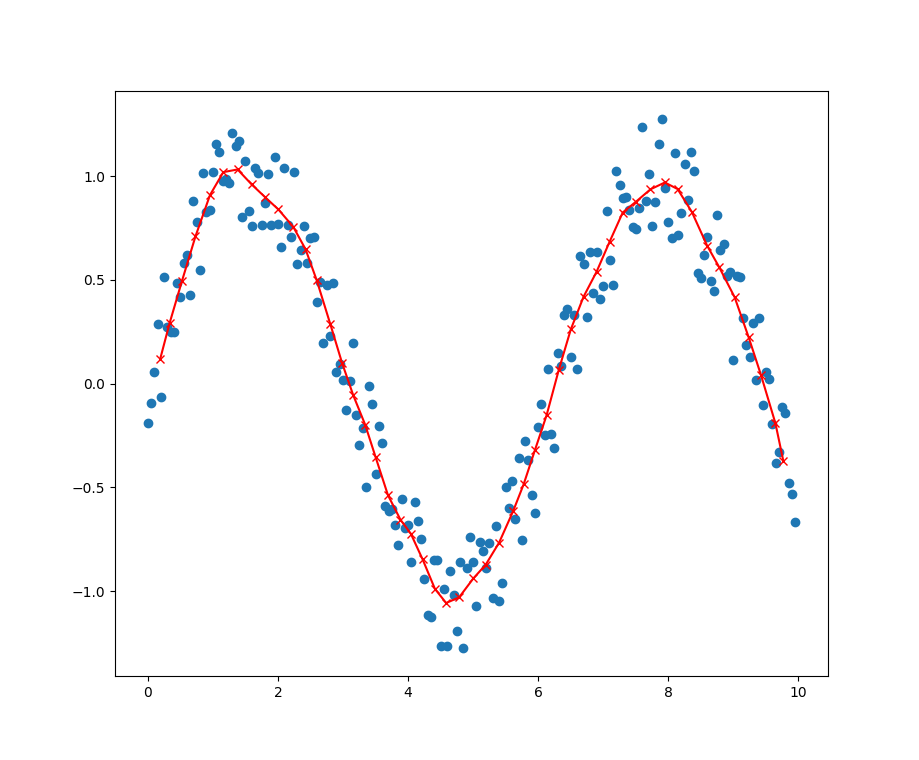
\includegraphics[scale=0.5]{Figures/som-implementation-example.png}
\decoRule
\caption[Ejemplo de salida de \glsentrytext{som}]{Ejemplo de salida de \glsentrytext{som}. Implementación propia.}
\label{fig:som-impl-example}
\end{figure}

\begin{figure}[th]
\centering
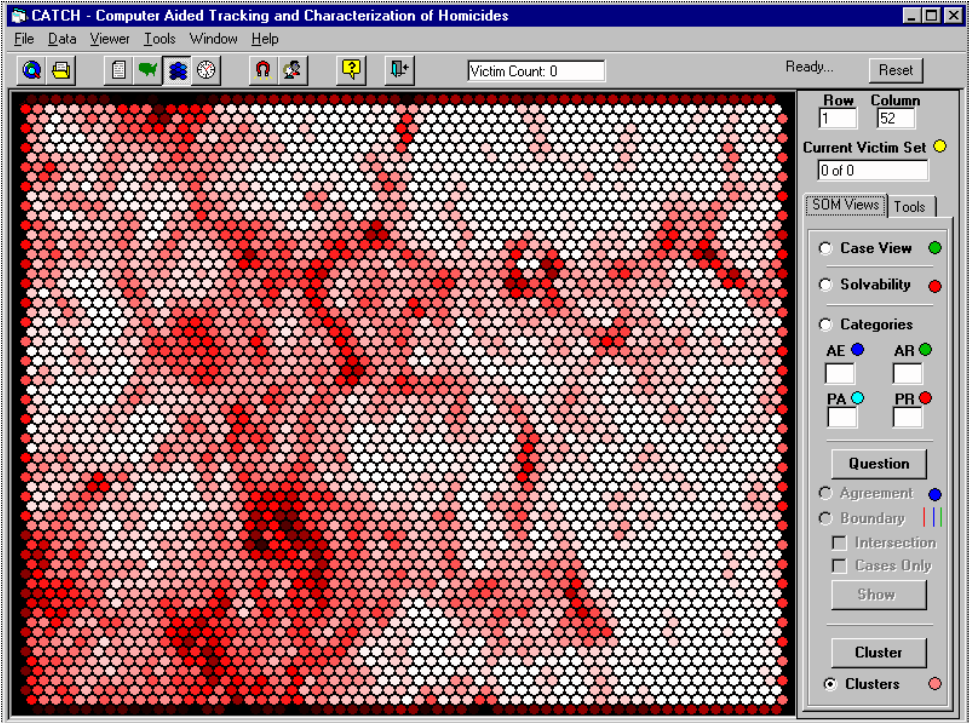
\includegraphics[scale=0.3]{Figures/som-example.png}
\decoRule
\caption[Ejemplo de uso de \glsentrytext{som} en aplicaciones de perfilado]{Ejemplo de uso de \glsentrytext{som} en aplicaciones de perfilado. Tomado de \cite{mena2003investigative}}
\label{fig:som-example}
\end{figure}

% ================================================================

\section{Aprendizaje de maquina (\glsentrylong{machinel})} \label{sec:ML}
Pendiente